%
% File acl2015.tex
%
% Contact: car@ir.hit.edu.cn, gdzhou@suda.edu.cn
%%
%% Based on the style files for ACL-2014, which were, in turn,
%% Based on the style files for ACL-2013, which were, in turn,
%% Based on the style files for ACL-2012, which were, in turn,
%% based on the style files for ACL-2011, which were, in turn,
%% based on the style files for ACL-2010, which were, in turn,
%% based on the style files for ACL-IJCNLP-2009, which were, in turn,
%% based on the style files for EACL-2009 and IJCNLP-2008...

%% Based on the style files for EACL 2006 by
%%e.agirre@ehu.es or Sergi.Balari@uab.es
%% and that of ACL 08 by Joakim Nivre and Noah Smith

\documentclass[11pt]{article}
\usepackage{acl2015}
\usepackage{times}
\usepackage{url}
\usepackage{latexsym}
\usepackage{graphicx}
\usepackage{float}

%\setlength\titlebox{5cm}

% You can expand the titlebox if you need extra space
% to show all the authors. Please do not make the titlebox
% smaller than 5cm (the original size); we will check this
% in the camera-ready version and ask you to change it back.


\title{Given Users recommendations Based on Reviews on Yelp }

\author{
  Shuwei Zhang \\
  {\tt shuweiz@usc.edu} \\\And
  Maiqi Tang \\
  {\tt maiqitan@usc.edu} \\\And
  Qingyang Zhang \\
  {\tt qzhang56@usc.edu} \\\And
   Yucan Luo \\
  {\tt yucanluo@usc.edu} \\\And
  Yuhui Zou \\
  {\tt yuhuizou@usc.edu}
  }

\date{}

\begin{document}

\maketitle

\section{Project Domain \& Goals}
The of this model is to give old users of Yelp restaurant recommendations based on their previous reviews posted on Yelp.

Our group picked task1-c as our project topic. The non-NLP domain algorithm we use is item-based collaborative filtering in data mining, widely used in the item recommendation system. Meanwhile, we want to enhance the user matching , which is a significant step in item-based collaborative filtering algorithms with several NLP algorithms.

The data set we will use is the data set of user reviews on Yelp. We want to use several methods to do data cleaning and preprocessing. After that, we use these combined algorithms mentioned before to calculate the user’s review’s similarity instead of simply using the user's rating to do user matching. For example, if we found several users’ reviews are similar, then these users are matched. We would use these users’ ratings in the group and use a test data set to calculate accuracy. Finally, we will evaluate the performance of each method in each step which would lead to the best result. And using the best combination to train our model, giving a better outcome for users.

The problem we solved is the recommendation by user's rating cannot fit users' interests well. For example, if we use ratings to find a restaurant that chicken is juicy and its overall rating is exceptionally high, the system recommends it to the user. However, this user prefers chicken, which is overcooked. And we could not find a matched restaurant by rating or simple categories filter. Then we use the NLP algorithm to analyze reviews' similarity. If the recommendation system could find a restaurant's reviews that are similar to the user's old review, this restaurant can better fit the user's interest.

\section{Related Work}
Currently, recommendation systems are broadly classified into collaborative filtering (CF) and content-based filtering (CB) (Park et al. 2011). The fundamental assumption is that if users A and B rate k items similarly, they share similar tastes or preferences, and hence will rate other items similarly (Goldberg et al. 2001). In many recent recommendation system projects, the testing RMSE has already been lower than 1.5. For example, on Kaggle competition (RecSys2013: Yelp Business Rating Prediction), the best testing RMSE is 1.19 eight years ago.
\begin{figure}[H]
\centering
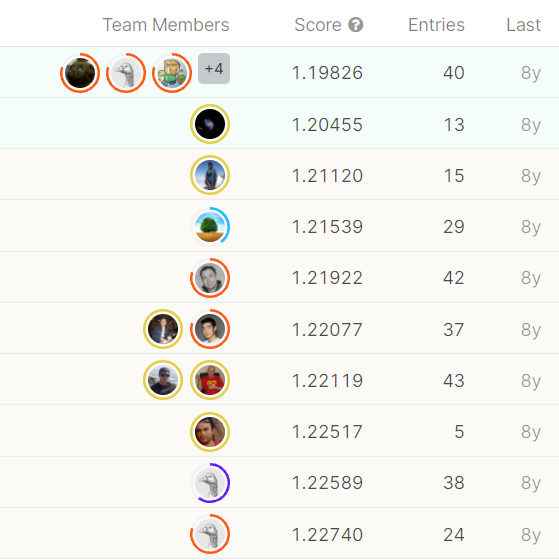
\includegraphics[width=0.5\textwidth]{kaggle.jpg}
\caption{Kaggle competition leaderboard}
\label{Fig.main2}
\end{figure}
Even on highly sparse data (99.98\% sparsity), Chen’s CF model has reached 1.1237 testing RMSE (Chen et al. 2012).

Sometimes, users do not want to try some recommended “similar” restaurants, but they want to try some fantastic restaurants that are not in their preference. Most recommendation systems that are based on CF or CB heavily rely on the similarities of preferences or taste which results in a lower rating for restaurants out of user’s preference. As a result, for users who do not want to have the same kind of food or the same kind of environment, these recommendation systems cannot exactly provide new restaurants out of users’ comfort zone.

We want to build a CF recommendation system based on sentiment analysis (SA) on historical reviews to find both the similarities and the differences. The goal is to better understand the characteristics of both customers and restaurants. So, the model can both provide restaurants that are under users’ preference and some new kinds of restaurants that are worthy to try. For reviews, we will try different pre-process and embedding skills, such as CBOW, Skip-Gram, or FastText, to convert review text to vectors. And then we will apply SA to identify the important features or attitudes for each review. Lastly, we will try different CF algorithms to provide more precise recommendations.

\section{Data}

In order to build a text-based recommendation system, we need to find a data set that records reviews and rating toward restaurants. Fortunately, Yelp has established a well-organized streamed database \footnote{Yelp Data set documentation url: \url{https://www.yelp.com/data set/documentation/main}} that provides reviews and ratings from customers, and the information about the restaurants those reviews are about. In this database, all the data is stored in JSON format with consistent schemas. The data set that we will mainly work on is the review data set, which provides the reviews from users to business; and the business data set, which provides the information of business listed on Yelp. In the reviews data set, we will mainly work with following attributes: business\_id, which is unique for each business listed on Yelp; text, which the review left to this restaurant; and stars, which is the rating left by the reviewer. For the business data set, we will use the business\_id from the reviews data set to match to the reviewed business. Then we can use the information from the business data set to tag and group up business.

The review data set had over 8 million instances, and it is hard to load all the data at once due the limitation of our computation resource. Therefore, we will utilize the business data set and apply some data mining algorithms to split the data set to reduce the size and avoid the biased data set. We will use some data mining tool, like Pyspark, to load and process the data parallelly. Afterward, we will shuffle and split the data set into a 4: 1 train and test partition. For the text part, we will first do the data clean to remove the unnecessary characters and do the contractions for the text. Meanwhile, the vocabularies used in the review are not alway correct. Therefore, we will use the spell corrector library in python to correct the spelling and reduce the vocabulary size. Also, another challenge is raised by the length of each review, which varies from 1 word to a long paragraph. Therefore, we will find a threshold to truncate the long review to increase the efficiency of feature extraction.


\section{Technical Challenge}

1. Contextual word and phrases homonyms. When we compare two sentences with semantic similarity, it is possible to pair two different meanings of sentences which contain the same words into one cluster. While NLP language modeling can learn different meanings and definitions, differentiating between them in context can still present problems.

2. Irony and sarcasm. Language models usually interpret words or phrases, it can be positive or negative. However, in fact, the words or phrases actually connote the opposite.

3. Grammar error in text. Misused words and wrong sentence structure can also cause problems for sentence text analysis. Although we can use grammar correction to alleviate this problem, the correction will not be perfect.

4. Misspelled word. The Misspelled word will cause inaccuracy of performance. Even though there are some algorithms to correct misspelled words, the correction will not be accurate because the choice of correct word only depends on the misspelled word but not the understanding of the whole sentence.

5. Colloquialisms and slang. Informal phrases, expression, idioms, and culture-specific lingo also present problems for language modeling. Furthermore, cultural slang is constantly morphing and expanding, so new phrases and words pop up every day. It is hard for a formal language model to distinguish new words and phrases.

6. For some reviews, it is too short to perform language analysis. One option to solve the problems is padding the shorter reviews or treat it as the outlier and remove it.

7. New users can also present problems. Our model aims to find similar reviews and then recommend restaurants to users who share similar tastes. But it cannot recommend any restaurant to new users based on similarity, since they may not have any reviews yet. We can tackle this problem by implementing the content based analysis, which is a data mining technical.

8. Large datasets cause scale problems. The data set had over 8 million instances, so the training process will take a long time. Especially we need to train different models and each with different parameters.

9. Users with limited available reviews. Assume if the similarity of sentiment analysis vectors is greater than a threshold, then the users of those reviews are similar users. After data preprocessing and cleaning, it is possible that there is no similar user of the predicted user, and we cannot apply collaborative filtering in this case.

By combining BERT For Measuring Text Similarity with sentence similarity check using item based collaborative filtering, it might provide a better way to capture similarity between reviews. Furthermore, we can do sentiment analysis towards the restaurant based on customers' review, if two customers have same sentiment towards a same restaurant, it is possible that they have similar taste. Finally we can evaluate our model using customer rating. if we predicted that those customers have similar taste, then, they would give same restaurant similar rating.

% include your own bib file like this:
\bibliographystyle{acl}
\bibliography{acl2015}

\begin{thebibliography}{}

\bibitem[\protect\citename{Park \bgroup et al.\egroup}2011]{Park:11}
Park, Deuk Hee, et al.
\newblock 2011.
\newblock {\em A Review and Classification of Recommender Systems Research. International Proceedings of Economics Development \& Research 5.1}.

\bibitem[\protect\citename{Goldberg \bgroup et al.\egroup}2001]{Goldberg:01}
K. Goldberg, T. Roeder, D. Gupta, and C. Perkins,
\newblock 2001.
\newblock {\em Eigentaste: a constant time collaborative filtering algorithm, Information Retrieval, vol. 4, no. 2, pp. 133–151}.

\bibitem[\protect\citename{Chen \bgroup Posch \egroup}2012]{Chen:12}
P. Chen, D. Posch.
\newblock November 2012.
\newblock {\em Collaborative Filtering on Very Sparse Graphs, A Recommendation System for Yelp.com}.

\bibitem[\protect\citename{Prem Melville \bgroup Raymond J. Mooney \bgroup Ramadass Nagarajan}2002]{Melville: 2002}
Prem Melville, Raymond J. Mooney, Ramadass Nagarajan 
\newblock July 2002
\newblock {\em Content-Boosted Collaborative Filtering for Improved Recommendations}

\end{thebibliography}

\end{document}
